%! Author = arqfa
%! Date = 8/8/2023

% Preamble
%\documentclass[11pt]{article}
\documentclass[final,5p,times]{elsarticle}
% Packages
%% The amssymb package provides various useful mathematical symbols
\usepackage{amssymb}
%% The amsthm package provides extended theorem environments
\usepackage{amsthm}
\usepackage{graphicx}
\usepackage{tabularx}
\usepackage{booktabs}
%% The lineno packages adds line numbers. Start line numbering with
%%\begin{linenumbers}, end it with \end{linenumbers}. Or switch it on
%% for the whole article with \linenumbers
\usepackage{lineno}
\modulolinenumbers[10]
\usepackage{enumitem}

\usepackage{multirow}

\usepackage{caption}

\journal{Computer Aid Design}


% Document
\begin{document}

\begin{frontmatter}


\title{Embracing Complexity: Mixed Reality Assessment of User Tolerance for Complex Facades in Future Construction Trends}

%% use optional labels to link authors explicitly to addresses:
%% \author[label1,label2]{}
%% \affiliation[label1]{organization={},
%%             addressline={},
%%             city={},
%%             postcode={},
%%             state={},
%%             country={}}
%%
%% \affiliation[label2]{organization={},
%%             addressline={},
%%             city={},
%%             postcode={},
%%             state={},
%%             country={}}

\author[inst1]{Fabian Jarrin}
\author[inst1]{Yasuko Koga}
\author[inst2]{Diego Thomas}

\affiliation[inst1]{organization={Graduate School of Human-Environment Studies, Department of Architecture and Urban Design, Kyushu University},%Department and Organization
            addressline={744 Motooka, Nishi Ward},
            city={Fukuoka},
            postcode={819-0382},
            state={Kyushu},
            country={Japan}}

\affiliation[inst2]{organization={Graduate School of Information Science and Electrical Engineering, Kyushu University},%Department and Organization
            addressline={744 Motooka, Nishi Ward},
            city={Fukuoka},
            postcode={819-0382},
            state={Kyushu},
            country={Japan}}

\begin{abstract}
%% Text of abstract
%!Asbtract guidelines
        %A concise and factual abstract (100-150 words ) is required. The abstract should state briefly the purpose of the research, the principal results and major conclusions. An abstract is often presented separately from the article, so it must be able to stand alone. For this reason, References should be avoided, but if essential, then cite the author(s) and year(s). Also, non-standard or uncommon abbreviations should be avoided, but if essential they must be defined at their first mention in the abstract itself.



% check
% new version under reviewer guidelines: Abstracts should contain only 6 short sentences: 1) What is the problem being addressed? 2) What is the research question being asked? 3) What is the methodology being used to answer the stated research question? 4) What are the results obtained? 5) What is the meaning and importance of these results? 6) What are the directions for follow-up research?


Architectural practice is evolving through digital fabrication, enabling complex designs that challenge the uniformity of barren walls and fully glazed facades that often dominate contemporary streetscapes.
This study investigates user tolerance and acceptance of complex facades using Virtual Reality (VR) and Computer Vision through the Computational Image Complexity Analysis (CICA) system.
We applied VR simulations and CICA to quantitatively and qualitatively assess reactions to various facade complexities.
Results reveal a preference for moderate complexity, suggesting an ideal balance between simplicity and intricacy.
This highlights the importance of aligning architectural complexity with user preferences to enhance sustainability and satisfaction.
Future research should explore the long-term impact of complex facades on user well-being and environmental sustainability.


%version 2024/05
%This research uses virtual reality (VR) assessment and computer vision to explore complexity in architectural facade design.
%We aim to examine user tolerance and acceptance of complex facades, providing insights for future construction practices.
%A literature review confirms a trend towards increased complexity, preferring richly detailed facades with elements at various scales or materials with fractal qualities, diverging from modernist minimalism.
%We introduce the Computational Image Complexity Analysis (CICA) system to quantify this trend, revealing an upward complexity trajectory since the late 20th century.
%A VR experiment indicates a user preference for moderate complexity, suggesting a balance between intricacy and simplicity.
%Discrepancies between participant perceptions and CICA rankings highlight the subjective nature of complexity perception.
%Qualitative data suggests a shift towards customizable, user-responsive designs.
%Overall, the study underscores a shift towards embracing complexity in facade design, emphasizing the need for a balanced approach that aligns with user preferences and cultural contexts.

% version 2024/04
%This research uses virtual reality (VR) assessment, and computer vision to understand complexity in architectural facade design.
%We aim to examine user tolerance and acceptance of complex facades, providing insights for future construction practices.
%A literature review confirms a contemporary trend towards increased facade complexity, moving away from modernist minimalism.
%We introduce the `Computational Image Complexity Analysis' (CICA) system to quantify this trend, revealing an upward complexity trajectory since the late 20th century.
%A VR experiment indicates a user preference for moderate complexity, suggesting a balance between intricacy and simplicity in future architectural trends.
%Discrepancies between participant perceptions and CICA rankings highlight the subjective nature of complexity perception.
%Qualitative data suggests a shift towards customizable, user-responsive designs.
%Overall, the study underscores a contemporary shift towards embracing complexity in facade design, emphasizing the need for a balanced approach that aligns with user preferences and cultural contexts.



%previous
%This paper examines user perceptions and acceptance of complex facade designs in contemporary architecture, integrating digital fabrication, virtual reality (VR), and computer vision.
%Our research aims to shed light on the evolving trends in construction design.
%A literature review reveals a historical oscillation between simplicity and complexity in architectural styles.
%We introduce the `Computational Image Complexity Analysis' (CICA) method to quantitatively evaluate the complexity of building facades.
%This approach verifies a noticeable trend towards greater complexity since the late 20th century.
%In our VR experiment, participants evaluated various facades, expressing a preference for designs with a CICA complexity score of 3.82 out of 10.
%Subsequent surveys indicated a positive reception towards intricate designs, with an average rating of 4.9 on a 7-point scale.
%These outcomes align with our architectural analysis, indicating a continuing trend towards increased complexity in modern architectural design.




\end{abstract}


%%Graphical abstract

\begin{graphicalabstract}
    \centering
    \includegraphics[width= \textwidth, trim = 0 80 0 80, clip]{Images/GraphicAbstract}
    \label{fig:graphic_abstract}
\end{graphicalabstract}

%%Research highlights
\begin{highlights}
%highlights
% highlights
% These bullet points should capture the novel results of your research as well as new methods that were used during the study (if any).
% Think of them as the "elevator pitch" of your article. Please include terms that you know your readers will be looking for online. Don't try to capture all ideas, concepts or conclusions as highlights are meant to be short:
% 85 characters or fewer, including spaces.


\item Architectural design faces challenges in quantifying facade complexity effectively.
\item CICA system developed using VR and Computer Vision to assess facade complexity.
\item CICA system aids in historical trend analysis of architectural complexity.
\item Findings show a 9\% deviation between CICA system complexity scores and user perceptions.
\item Study highlights user preference for moderate complexity, balancing design intricacy.


%previous iteration
%\item Investigates VR and CV methods for quantifying facade complexity in architectural design.
%\item CICA system integrates VR and CV to measure complexity and align with user perceptions.
%\item CICA system aids in historical trend analysis of architectural complexity.
%\item Study reveals an average 9\% deviation between system measurements and user perceptions.
%\item Findings show preference for moderate complexity, balancing simplicity and intricacy.


\end{highlights}

\begin{keyword}
%% keywords here, in the form: keyword \sep keyword
Data-driven design\sep Complex Facades \sep Mixed Reality Assessment \sep Architectural Aesthetics\sep Technological Innovation\sep

\end{keyword}

\end{frontmatter}
%\linenumbers
%\modulolinenumbers[10]
%
\begin{linenumbers}


\section{Introduction}
\label{sec:1Introduction}
%%State the objectives of the work and provide an adequate background, avoiding a detailed literature survey or a summary of the results.
%%Introduction

%=================================
%%Reference
%%https://www.scribbr.com/research-paper/research-paper-introduction/
%%State the objectives of the work and provide an adequate background, avoiding a detailed literature survey or a summary of the results.

%Step1. Introduce your topic.
     %This is generally accomplished with a strong opening hook.
%Step2. Describe the background.
     %For a paper describing original research, you’ll instead provide an overview of the most relevant research that has already been conducted.
%Step3. Establish your research problem.
     %In an empirical research paper, try to lead into the problem on the basis of your discussion of the literature.
%Step4. Specify your objective(s).
     %The research question is the question you want to answer in an empirical research paper. If your research involved testing hypotheses, these should be stated along with your research question.
%Step 5: Map out your paper.
     %The final part of the introduction is often dedicated to a brief overview of the rest of the paper.

%recommended limit 500 words
%=================================

Recent advancements in Building Information Modeling (BIM) and digital fabrication are transforming architectural practice.
These technologies enable architects to design intricate and complex forms, moving beyond the uniformity of barren walls and fully glazed facades that often dominate contemporary streetscapes.
By leveraging these advancements, architects can introduce complexity and detail into their designs, enhancing both the visual and functional aspects of buildings, and creating more engaging and dynamic environments that potentially redefine the relationship between form and function~\cite{Leach2016}.

\deleted{
However, the pursuit of complexity in architectural design must be balanced with sustainability and user satisfaction.
Designs that are overly complex without consideration of these factors can quickly become outdated and disconnected from their inhabitants, leading to issues of obsolescence and lack of relevance~\cite{Oberfrancova2021}.
Understanding how complexity can enhance both environmental sustainability and user satisfaction is therefore crucial for modern architectural practice.
}

\added{
However, the pursuit of complexity in architectural design must be balanced with sustainability and user satisfaction.
Overly complex designs, when not thoughtfully integrated, can quickly become outdated, contributing to obsolescence and construction waste, a major source of carbon emissions~\cite{Oberfrancova2021}.
By incorporating complexity analysis into the design process and controlling and optimizing facade complexity, architects can create designs that are not only visually engaging but also adaptable and long-lasting, reducing the need for frequent renovations and replacements.
}

\added{
Understanding the complexity of facade designs is crucial because facades are the most visible part of a building, playing a significant role in urban aesthetics and user perception. Designs that strike the right balance between simplicity and complexity can create environments that are not only visually stimulating but also comfortable and functional for occupants~\cite{Browning2014}. Complexity can enhance the user experience, making facades more engaging and improving user satisfaction with the built environment. Moreover, facade design can contribute to energy efficiency and material optimization, especially when combined with advanced technologies like digital fabrication and parametric design.
}

\added{
This study proposes the development of a system to measure and adjust facade complexity, which could be integrated with existing tools for energy efficiency, material optimization, and environmental comfort.
Such an approach could significantly minimize environmental impact while addressing the sustainability challenges in modern construction.
Understanding how complexity can enhance both environmental sustainability and user satisfaction is therefore crucial for modern architectural practice.
}

\deleted{
Previous research has extensively explored the impact of complexity in architectural design, identifying mathematical relationships between complexity and aesthetic value ~\cite{Bies2016, Douchova2016, Redies2015}.
Despite these insights, the architectural field has yet to develop frameworks that leverage these principles for practical design applications, especially considering modern technological advancements aimed at sustainability.
}

\added{
Previous research has extensively explored the impact of complexity in architectural design, identifying mathematical relationships between complexity and aesthetic value ~\cite{Bies2016, Douchova2016, Redies2015}. Despite these insights, the architectural field has yet to develop frameworks that leverage these principles for practical design applications, especially considering modern technological advancements such as digital fabrication and parametric design. These technologies not only enable the creation of complex forms but when paired with `Data-driven Building Design' (DBD) optimization they also support energy efficiency, material reduction, and long-term sustainability.
}

This study aims to bridge the gap between theoretical understanding and practical application by developing a methodology to measure facade complexity.
The objectives are to generate data that can improve DBD by integrating a complexity scoring function that can inform on the optimal rate between simplicity and complexity based on historical analysis and user preferences.
By integrating complexity insights with modern technological applications, we seek to provide actionable, data-driven insights for future architectural practices promoting the advancement aimed at sustainability.

The methodology is structured around 4 primary components:

\begin{enumerate}
    \item Literature review: Significant studies on the foundational theories of complexity, and an exploration of the fluctuation between simplicity and complexity in architectural history.
    \item Complexity Analysis System Development: \deleted{Implements a Virtual Reality (VR) framework, and combines it with a Computational Image Complexity Analysis (CICA) component using computer vision (CV) algorithms to quantitatively assess the complexity of facade designs.}\added{This component integrates a Virtual Reality (VR) framework with the Computational Image Complexity Analysis (CICA) system, specifically developed for this study. The CICA system utilizes computer vision (CV) algorithms to quantitatively assess facade design complexity.}
    \item Experiment Execution: involving VR to facilitate participant interaction with complex facades, augmented by surveys and interviews for qualitative insight.
    \item Data Analysis and Validation: Assessing the data collected during the experiment to evaluate the effectiveness of the Complexity Analysis System and CICA framework in measuring complexity and user preferences.
\end{enumerate}

This comprehensive approach aims to enrich our understanding of facade complexity and its role in the contemporary Architectural, Engineering, and Construction (AEC) industry.



\section{Theory Framework}
\label{sec:Theory Framework}
%% Research Background

%% A Theory section should extend, not repeat, the background to the article already dealt with in the Introduction and lay the foundation for further work. In contrast, a Calculation section represents a practical development from a theoretical basis.

%A theoretical framework is a foundational review of existing theories that serves as a roadmap for developing the arguments you will use in your own work.

%=============================================================================
%Outline.
%1. Introduction
%2. The importance of facade in a building.
%3. A brief analysis of architecture styles and the
%3. A reflexion into digital fabrication techniques specially parametric design.
%4. The principle od data driven design.
%5. An analysis into mixed reality and the advantages of introducing this  into the design review.
%=============================================================================

%///////////////////////////////////////////////////////////////
%% refined outline of theory framework

%6. **Human-Centric Design Philosophy:** Explore the historical evolution of architectural philosophies that prioritize human experience and well-being. Discuss how different architectural styles and movements have addressed the balance between ornamentation, functionality, and human comfort.

%7. **Cultural Significance of Facades:** Delve deeper into how facades reflect cultural values, societal norms, and historical contexts. Explore how different societies and civilizations have expressed their identity through architectural ornamentation and symbolism.

%8. **Environmental Sustainability:** Investigate how the integration of complex facades and digital fabrication aligns with contemporary sustainability principles. Examine how parametric design and data-driven approaches can enhance energy efficiency, reduce material waste, and contribute to sustainable construction practices.

%9. **Ethics and Social Responsibility:** Consider the ethical implications of embracing ornate designs and digital fabrication in a world grappling with issues of resource scarcity and inequality. Discuss how responsible architectural practices can address these challenges and contribute positively to society.

%10. **Collaborative Design Process:** Explore the collaborative aspects of architectural design when utilizing digital fabrication and mixed reality. Discuss how these technologies foster interdisciplinary collaboration among architects, engineers, urban planners, and other stakeholders.

%11. **Challenges and Limitations:** Address the potential challenges and limitations of implementing complex facades and digital fabrication techniques. Discuss technical, economic, and cultural barriers that may arise and the strategies to overcome them.

%12. **Case Studies and Success Stories:** Showcase real-world examples of projects that have successfully integrated complex facades, digital fabrication, and mixed reality. Analyze the impact of these projects on user experience, urban aesthetics, and architectural innovation.

%13. **User-Centered Design:** Delve into the principles of user-centered design and human factors that influence the acceptance of intricate facades. Consider factors like psychological comfort, emotional response, and sensory experience in relation to complex architectural designs.

%14. **Cognitive Aspects of Mixed Reality:** Explore the cognitive psychology behind mixed reality experiences and how they influence user perceptions of architectural complexity. Consider how elements like immersion, presence, and interaction affect users' understanding and appreciation of design.

%15. **Future Trends and Speculation:** Speculate on the potential future trajectories of architectural design, digital fabrication, and mixed reality. Discuss how these trends might shape the built environment, and propose ideas for further research and exploration.

%By incorporating these additional topics into your theory framework, you can provide a comprehensive and well-rounded context for your research, offering deeper insights into the historical, cultural, ethical, and technological dimensions of complex facades, digital fabrication, and mixed reality in architecture.
%///////////////////////////////////////////////////////////////

%% Introduction

Architecture, as a reflection of society, has continually evolved to accommodate the needs of the communities it shelters.
Buildings, in essence, serve as tools with a purpose—guardians of societies, nurturers of generations, and manifestations of future aspirations.

Critique is inherent to architecture, and it falls upon successive generations to discern flaws within the inherited built environment.
Amidst these legacies, the legacy of the modernist movement, emerging in the mid-20th century, emerges as particularly relevant.
Anchored in principles of simplicity and the maxim ``form follows function'', this movement gained global prominence, addressing urbanization challenges triggered by rural migration to cities.

Yet, this era's legacy brings forth a profound debate.
While remarkable creations emerged, it's important not to label nearly a century of architectural style as universally negative.
However, society acknowledges the unintended consequences.
The fervor for uniformity and minimalism, epitomized by modernism, led to a disconnect from cultural roots.
As cities embraced this discourse, they lost distinct identities, homogenizing urban landscapes and erasing their unique memories.

This realization underscores the complex narrative of architecture—a dynamic interplay between innovation, utility, and cultural heritage.
It reminds us that while architectural styles may have their merits, the preservation of cultural essence and identity is vital for thriving urban spaces that resonate with inhabitants and stand the test of time.

 Because as Gage~\cite{Gage2015} eloquently puts it ``If architecture is to exist in the 21st century, when attention is focused on the fast-paced worlds of technology, fashion, and entertainment, it must not recede into the background as mere functional equipment''.

As we delve into the theory framework that underpins this research, we embark on a journey through historical shifts between architectural complexity and simplicity.
We explore the significance of facades in shaping the identity of structures.
We reflect on the integration of digital fabrication techniques, particularly parametric design, and the fundamental principles of data-driven design.
Our exploration extends to the realm of mixed reality and the promising advantages it introduces to the architectural design review process.

Each component within this theory framework contributes to our understanding of the intricate interplay between architectural evolution and societal dynamics.
As we navigate through complexities and contemplate the subtleties of design paradigms, we seek to uncover insights that illuminate the path to a more harmonious relationship between built environments and the people who inhabit them.

\subsection{Human-Centric Design Philosophy across the history of architecture styles}
\label{subsec:TimelineArchitectureStyles}

%%Human-Centric Design Philosophy: Explore the historical evolution of architectural philosophies that prioritize human experience and well-being. Discuss how different architectural styles and movements have addressed the balance between ornamentation, functionality, and human comfort.


Architecture stands as a unique art form, setting itself apart from other creative mediums.
It requires not only the transformation of the ordinary into the extraordinary, akin to painting and sculpture, but also the imperative to fulfill the purpose and functionality of a building\cite{Hnin2022}.

At the core of architectural evolution resides a dynamic interplay between simplicity and complexity, often guided by the intersection of societal values and technological advancements\cite{Economakis2023}.
However, it's important to clarify that within the context of this research, neither simplicity nor complexity carry any inherent negative or positive connotations.
Using the term ``simplicity`` here doesn't imply a condemnation of one style in favor of another;
rather, it highlights that throughout the history of architecture and its various styles, there have been periods characterized by evident complexities as well as phases where designs embraced apparent simplicities that hid their intricacies into themselves.
Undoubtedly, every prevailing architectural style of its time has contributed masterpieces to the built environment.

Consider, for instance, the transition from the robust Romanesque classic style of the 10th century, notably exhibited in churches, to the Gothic style brought by groundbreaking advancements of the 12th century that introduced buttresses, revolutionizing load distribution\cite{Arora2023}(see Figure\ref{fig:RomanesquevsGothic}).
This innovation propelled churches skyward, inviting luminous interplays to embellish the interiors through stunning stained-glass windows bedecked in intricate design\cite{Stacbond2020}.

This trend resurfaced as time unfolded, transitioning from the complex Gothic style to the revival of Greek and Roman ideals, exemplified by the symmetrical perfection of the Renaissance era in the 14th century.
This resurgence was succeeded by the opulent ornamentation of the Baroque style in the 16th century, followed by the neoclassical revival of the 18th century, heavily influenced by classical Greek and Palladian architecture.

In the 1920s and 30s, the intricate Art Deco movement emerged, celebrating technological progress through luxurious materials and patterns seamlessly integrated with modern design and manufacturing techniques.
In response to this progression, the first half of the 20th century witnessed the emergence of Modern Architecture and rationalism.

This architectural ethos adopted the maxim ``Form follows function'', emphasizing functionalism and characterized by a rejection of traditional ornament in favor of new forms of more subtles intricacies like the “aesthetics of machinery” that showcased architecture  enriched  with  only  the  beauty of its lines and the use of new-age materials such as steel, glass, and concrete\cite{Gage2015}(see Figure\ref{fig:ArtDecovsModernism}).
The postmodernism style of the late 60's marks a radical return of ornament in form recognizing that even simplified modern elements serve as ornamentation focusing on the thought of freeing design element from oppresive modern constraints.
The  beginning  of  the  1980s marked a shift towards more imaginative and expressive architecture following architects like Frank Gehry, Zaha Hadid and Rem koolhaas who treated their constructions as monuments of Ornament that transformed architecture into a media.
With highly complex shapes brought into reality by the incorporation of digital technologies.
Examples abound in this era ranging form justaposition of complex ornaments over simple facades to the transformation of ornament not as an articulate material, but as a form of structure, turning the structure to building and ornament.
However due to the complex fabrication that such examples require and expertise, they are not a part of the urban fabric but rather sporadic cases across the globe which can truly be considered as the defining contemporary style, however the democratization of digital fabrication could bring the tools require to create said structures around the world diversifying among cultures and providing authentic interpretations of their context express in the form of complex buildings. This is the time of complexity and ornament.

``If architecture is to exist in the 21st century, when attention is focused on the fast-paced worlds of technology, fashion, and entertainment, it must not recede into the background as mere functional equipment''\cite{Gage2015}.


\subsection{Cultural Significance of Facades and Ornament}
\label{subsec: FacadeandOrnament }
The resonance of Louis Sullivan's renowned phrase, ``Form follows function,`` throughout the Modernist movement of the 20th century and its continued influence on subsequent decades can be attributed to the pivotal role of a building's purpose and functions as the genesis and core of a project\cite{Hnin2022}.

This principle found its radicalization within the context of the times, partly due to a prevailing stance against ornamentation, often dismissed on moralistic grounds.
This sentiment deemed everything beyond function as secondary, exemplified by works like Adolf Loos' 1908 article ``Ornament and Crime,`` which advocated for functional design by condemning traditional ornamentation as superfluous\cite{Saglam2014}.

Even during this era when ornamentation was viewed unfavorably, prominent figures of the time, such as Le Corbusier, who publicly championed the functional ideology, would ingeniously devise methods to infuse their creations with a distinct form of ornamentation, albeit one rooted in materials' textures, structural elements, and inventive ways of articulating functionality.\cite{Saglam2014}.
In Venturi's opinion\cite{Venturi1972} 1960's ``Modern architecture uses expressive ornament and shuns explicit symbolic  ornament'' and all the simplistic facades are a type of ornament\cite{Saglam2014}.

          ``If architecture is to exist in the 21st century, when attention is focused on the fast-paced worlds of technology, fashion, and entertainment, it must not recede into the background as mere functional equipment''\cite{Gage2015}.

          According to Krier the mature city achieves balance with nature and with the people that it serves in its scale, size and integration of residential, commercial and civic functions.
          Krier argues that the reconstruction of a city is a moral imperative, a global project that it is at once cultural social economic and ecological. Time of video 1:06:29

We evidence this when observing the Romanesque classical style on the 10 th century found mostly in churches ith thick wall structures, followed by the breakthrough in load distribution during the Gothic style of the 12th to the 16th century which abandons the robustness to erect high buildings with complex great stained windows.
The Renaissance follows at the end of the Middle Ages and with it the return of the classical order with round arch and classical order columns that brings ornaments back to the interior in favour of more simplified exteriors.
In reaction to this style Baroque style surges with more dynamic forms , irregular shapes and exaggerated ornamentation in bold combinations.

%%%%
what initially motivates this research is the conscious realization that
Upon delving into the annals of influential architectural styles, a discernible pattern emerges—an oscillation between simplicity and complexity(see Figure\ref{fig:TimelineArchitecture}).
This recurrent cycle in architectural paradigms is not only reflective of the values ingrained in the societies they house, but also closely tied to pivotal technological advancements.
Consider, for instance, the transition from the Romanesque style of the 10th century to the Complex Gothic style 12th style, replaced by the revival of greek and roman ideals during the Renaissence style, followed by the complex opulent ornamentation of the Baroque style in the 16th century replaced by the neoclassical revival of the 18th century, heavily influenced by classical Greek and Palladian architecture\cite{Arora2023}.
This pattern repeats all the way to the 1920s and 30s, the intricate Art Deco will be replaced on the first half of the 20th century witnessed the emergence of Modern Architecture and rationalism emphasizing functionalism and minimalistic architecture




This shift encapsulates the quintessence of architectural evolution—an ever-changing interplay between simplicity and complexity, often steered by the confluence of societal values and technological breakthroughs.


Once again, we find ourselves at a pivotal juncture in history, as the emergence of computer-aided design converges with the industrialization of construction, ushering in a new paradigm in architectural design.
The 20th-century dominance of Rationalism, exemplified by figures like Le Corbusier, underscored an ethos of oversimplification and functionality.
Characterized by straightforward, symmetrical forms and concrete as the favored medium, this era yielded cities estranged from human-centric design.
Swift transportation took precedence, fracturing urban spaces that once defined vibrant societies\cite{Stacbond2020}.
Subsequently, industrial design asserted its dominance as the blueprint for future construction\cite{Economakis2023}, casting architecture in the mold of minimalism and mass-produced uniformity, forsaking the ornate allure and individuality of yesteryears.

\subsection{Object-Oriented Ontology}
\label{subsec:ObjectOrientedOntology}
% add the concept of Object-Oriented. Using these concepts as basis. I want to express that the mr experiment is based on the idea that architecture as a tool should be invisible and confortable while in use. But it should  create emotion when seen as part of the landscape as a form of art to recapture the humand oriented city .

Heideggers tool analysis states that as the tool is a tool it disappears in favor of some purpose he continues to explain that generally we don't notice equipment until it fails, like when An earthquake calls attention to the ground we walk or when a medical problem alerts us of the presence of organs that we have silently depended\cite{Harman2011}.
Harmans, Object-oriented ontology, borrows this concept to formulate its central claim that objects have hidden qualities and realities, and they withdraw from our understanding.\cite{Gage2015}
he idea that we live our lives on a layer of invisible equipment has significant ramifications for architecture, a discipline that produces the equipment on and in which we exist.\cite{Gage2015}

%% A Theory section should extend, not repeat, the background to the article already dealt with in the Introduction and lay the foundation for further work. In contrast, a Calculation section represents a practical development from a theoretical basis.
    \subsection{Human-Centric Design Philosophy across the history of architecture styles}
    \label{subsec:TimelineArchitectureStyles}
    
%\subsection{Human-Centric Design Philosophy across the history of architecture styles}
%\label{subsec:TimelineArchitectureStyles}

%===========================
%%Human-Centric Design Philosophy: Explore the historical evolution of architectural philosophies that prioritize human experience and well-being. Discuss how different architectural styles and movements have addressed the balance between ornamentation, functionality, and human comfort.
%===========================

Architecture stands as a unique art form, setting itself apart from other creative mediums.
It requires not only the transformation of the ordinary into the extraordinary, akin to painting and sculpture, but also the imperative to fulfill the purpose and functionality of a building\cite{Hnin2022}.

At the core of architectural evolution resides a dynamic interplay between simplicity and complexity, often guided by the intersection of societal values and technological advancements\cite{Economakis2023}.
However, it's important to clarify that within the context of this research, neither simplicity nor complexity carry any inherent negative or positive connotations.
Using the term ``simplicity`` here doesn't imply a condemnation of one style in favor of another;
rather, it highlights that throughout the history of architecture and its various styles, there have been periods characterized by evident complexities as well as phases where designs embraced apparent simplicities that hid their intricacies into themselves.
Undoubtedly, every prevailing architectural style of its time has contributed masterpieces to the built environment.

Consider, for instance, the transition from the robust Romanesque classic style of the 10th century, notably exhibited in churches, to the Gothic style brought by groundbreaking advancements of the 12th century that introduced buttresses, revolutionizing load distribution\cite{Arora2023}(see Figure\ref{fig:RomanesquevsGothic}).
This innovation propelled churches skyward, inviting luminous interplays to embellish the interiors through stunning stained-glass windows bedecked in intricate design\cite{Stacbond2020}.

This oscillation between complexity and simplicity persists through time— transitioning from the intricate Gothic style to the revival of Greek and Roman ideals, exemplified by the symmetrical perfection of the Renaissance era in the 14th century.

This resurgence was succeeded by the opulent ornamentation and exuberance of the Baroque style in the 16th century, essentially a creation of the Chatolic church, that started in Europe and later spread across the New world in other Chatolic nations.
It was characterized by the preference for curves over the straight line, an interest in complex plans and volumes, overlapping architectural forms, and an interest for combining the three arts of painting, sculpture and architecture\cite{Economakis2023}.

The progression continued with the classical revival of the 18th century, heavily influenced by the architectural principles of classical Greece and the Palladian style.
This revival aimed to create picturesque compositions and sought to reestablish the rational simplicity that defined ancient Greece and Rome\cite{Economakis2023}.

The late 18th century marked the beginning of globalization and an information explosion, which enabled scientific advancements but also blurred the geographical origins of architectural forms.
As a result, architectural expressions from diverse cultures became acceptable options in various contexts.
This phenomenon led to the incorporation of multiple historical references into buildings, soon Gothic, Oriental or even Egyptian styles, to name a few, were integrated into victorian houses, resulting in stylistic confusion known as Relativism and Subjectivism.
Architects grappled with a multitude of options and no clear consensus on architectural expression\cite{Economakis2023}.

In response to this architectural chaos, the Neoclassical style would appear, envisioned under the conservative academicism of the 19th century that aimed to bring order by consolidating the architectural profession under the teachings of classical architecture as idealized during the Renaissance.
Characterized by being bilaterally symmetrical and sel-referential or a-contextual with little regard to how they integrated to urban settings.
This heavily inspired greek and Palladian architecture would integrate with new technologies like reinforced concrete and cast iron.
Led by the École des Beaux-Arts in Paris, the Neoclassic style gained prominence and persisted until the early 20th century\cite{Economakis2023}.

However, by the late 19th century, the increasingly rigid academicism of the École des Beaux-Arts gave way to a shift towards ostentation.
The lack of volumetric hierarchy in building designs led to a departure from the sobriety and principles of the Renaissance.
Their monumentality originally praised was now resulting in a tendency towards overelaboration as buildings competed for attention\cite{Economakis2023}.

During this period The Art Deco movement would also make its appearance, flourishing in the 1920s and 30s, on a style that celebrated technological progress through luxurious materials and intricate patterns.
It blended modern design with artistic craftsmanship, embracing geometric shapes, bold colors, and streamlined forms.
Art Deco architecture often featured sleek lines, zigzags, and stylized motifs, capturing the spirit of the era's dynamism and opulence.\cite{Arora2023}

In response to the attitudes of the Ecole of Beaux Arts and its cult towards exuberance, an antagonism was formed specially among the more socially-minded ones and during the first half of the 20th century, society would witness the emergence of Modern Architecture and rationalism with their increasing radical approaches towards the built environment (see Figure\ref{fig:NeoclassicalvsModernism}).

%%Figure neoclassicim vs modernism
     \begin{figure}[htb]
          \centering
          \includegraphics[width= \linewidth]{Images/NeoclassicismVsModernism}
          \caption{Neoclassic building "Paris Opera" 19th AC (left) vs Modernist house "Villa Savoye" 20th AC (right). From Complexity to simplicity. (\textit{Images edited from source:\cite{Stacbond2020}})}
          \label{fig:NeoclassicalvsModernism}
        \end{figure}

This architectural ethos adopted the maxim ``Form follows function'', emphasizing functionalism and characterized by a rejection of traditional ornament in favor of new forms of more subtles intricacies like the “aesthetics of machinery” that showcased architecture  enriched  with  only  the  beauty of its lines and the use of new-age materials such as steel, glass, and concrete\cite{Gage2015}.
Venturi\cite{Venturi1972} further reflects that modern architecture considered as progressive, If not revolutionary, utopian, and puristic;
it  is  dissatisfied  with existing conditions and its architects would prefer to change rather than enhance what is there.

%% add some extra references to the modernist section specially about the urban configuration

The postmodernism style of the late 60's marks a radical return of ornament in form recognizing that even simplified modern elements serve as ornamentation focusing on the thought of freeing design element from oppresive modern constraints.



The late 20th century embraced imagination and expression through architects like Frank Gehry, Zaha Hadid, and Rem Koolhaas.
Their constructions stood as monumental expressions of ornament, enabled by digital technologies (Figure\ref{fig:Modernismvspostmodernism}).

%%Figure neoclassicim vs modernism
     \begin{figure}[htb]
          \centering
          \includegraphics[width= \linewidth]{Images/modernism vs postmodernism}
          \caption{Modernist building "Bauhaus School" 20th AC (left) vs Postmodernist "Guggenheim museum" 1997 (right). From simplicity to Complexity. (\textit{Images edited from source:\cite{Arora2023}})}
          \label{fig:Modernismvspostmodernism}
        \end{figure}

Intricate shapes and structures have materialized, spanning from juxtaposed ornaments to innovative transformative structural ornamentation.
This pursuit of complexity is a global phenomenon, prompting a competitive quest among leading contemporary architectural firms to harness parametric design as a tool to conceive groundbreaking new buildings.\cite{Burlando2019}.

However, due to their complexity, these structures remained exceptional, not integrated into the urban fabric.
Now at the beginning of the 21st century and the advent of the 4th industrial revolution, characterized by a fusion of technologies that is blurring the lines between the physical, digital, and biological spheres\cite{Schwab2016}, forecasts the democratization of digital fabrication which in turn will bring a paradigm shift, offering globally to all cultures the means to express authenticity through complex parametric designs, signaling a contemporary era embracing complexity and ornament.

Amidst this historical exploration, it becomes evident that the architecture of the future is poised to harmonize ornamentation, functionality, and human comfort.
The trajectory points towards a style of complexity—a style that crafts a delicate equilibrium, resonating with the values of our time and the technological possibilities at our fingertips.

In this intricate interplay, architecture emerges as a tangible synthesis of human experience and creative expression, balancing ornament's aesthetic allure, the essential functionality of the built environment, and the crucial comfort of its inhabitants.

    \subsection{Cultural Significance of Facades and Ornament}
    \label{subsec:FacadeandOrnament}
    
%!subsection{Cultural Significance of Facades and Ornament}
%!\label{subsec: FacadeandOrnament}

%!==========================
%Delve deeper into how facades reflect cultural values, societal norms, and historical contexts. Explore how different societies and civilizations have expressed their identity through architectural ornamentation and symbolism.
%!==========================
We have established a foundation for the notion that contemporary architecture is gravitating towards a renaissance of complexity.
This resurgence is catalyzed by the utilization of technology and sophisticated software analyses, enabling the creation of innovative ornamentation that seamlessly integrates functionality with cultural heritage.
This evolution paves the way for the elaboration of intricate patterns that serve as a powerful medium to express the distinct identity of the local environment, thereby rejuvenating the urban landscape.

Transitioning into the focal point of this research, we delve into the trajectory of architectural complexity within the specific realm of facades.

Facades, a paramount architectural element, have held an enduring significance for centuries due to their role as the initial point of contact with a building, acting as a boundary between the interior and the exterior, working as an interface between the living spaces and the external climate, influencing comfort and energy efficiency\cite{Kamal2020} thereby acting as the primary medium through which the structure interacts with its surroundings (Figure\ref{fig:FacadeBaroqueVsContemporary}).

%% Figure of baroque facade vs contemporary facade
     \begin{figure}[htb]
          \centering
          \includegraphics[width= \linewidth]{Images/BaroqueVsContemporaryfacade}
          \caption{Evolution of facade design.
          Baroque Facade 1639 by Bernini (left) vs Contemporary facade, building O-14 by Reiser + Umemoto, 21st Century (right) (\textit{Images edited from source)}}
          \label{fig:FacadeBaroqueVsContemporary}
        \end{figure}

However, much like the broader scope of architecture, the role of ornamentation and facades has also undergone evolution and transformation throughout history.
To elucidate how various societies and civilizations have conveyed their identity through architectural ornamentation and symbolism, we embark on an exploration of the interpretations given to facades by some of the most influential architects and artists of their respective eras.

%%Facade according to vitruvius

Vitruvius, a celebrated Roman architect and military engineer, in 1st century BCE, author of ``De Architecura'', a series of ten books considered as the first treatise in architecture theory\cite{Kruft1994}.
Within this work, Vitruvius advocates for three essential attributes that a building should embody: ``firmitas'' (structural soundness), ``utilitas'' (functionality), and ``venustas'' (beauty or aesthetics)\cite{Ostwald2023}.

Vitruvius places emphasis primarily on Reason, and secondarily on proportions.
It's worth highlighting that the cultural atmosphere in ancient Rome during the late first century B.C favoured the understanding of the world as a well-structured and ordered whole\cite{Lefas2000}.

Facades partake of this reasoning and in accordance to Vitruvius should not only be visually appealing but should also reflect the underlying structural integrity of the building and fulfill its intended purpose effectively(Figure\ref{fig:Vitruvianarchitecture}).
In terms of ornamentation, Vitruvius seeks to approach this subjective realm, dominated by taste, with objectivity.
He rationalizes that a pleasing appearance emerges from the harmony and balance among the components that constitute a composition\cite{Lefas2000}.

%% Figure of vitruvian Architecture
    \begin{figure}[htb]
        \centering
        \includegraphics[width= \linewidth]{Images/VitruvianArchitecture}
        \caption{Facade and ornament according to Vitruvius, with emphasis in order symmetry and harmony. Pantheon's facade (left) and cross section(right) symmetry analysis (\textit{Images edited from source)}}
        \label{fig:Vitruvianarchitecture}
    \end{figure}

Additionally, Vitruvius determines that the deciding factor for those components would follow the principle of ``Decor'',  the  fifth  principle on his system of values that elevates simple  building  practice  into  architecture, defined as the property that  deals  with  the  «appropriate»  articulation and construction of the work on principles respecting religion, nature and social conventions\cite{Lefas2000}.

In essence, according to Vitruvius, facades and their ornamentation stem from a sense of order and rationality.
They are achieved through a harmonious equilibrium of well-considered elements that adhere to established principles, while taking into account both tradition and nature.
This approach aims to achieve beauty while also effectively fulfilling the intended purpose of the facade.

Vitruvius's contributions would have a lasting impact on the field of construction spanning centuries.
However, his work remained largely dormant for a considerable period until its revival during the Renaissance, which encompassed the 14th to the 17th century.

This resurgence continued during the Neoclassical style of the 18th century and the Ecole des Beaux-Arts style of the 19th and early 20th centuries.
This series of revivals and reinterpretations led to the rekindling of Classical architecture in the years that followed\cite{Wikipedia2023}(Figure\ref{fig:ClassicismNeoClassicism}).

%% Figure of Classicism and Neo classicism facade
     \begin{figure}[htb]
          \centering
          \includegraphics[width= \linewidth]{Images/ClassicismNeoClassicism}
          \caption{Continuity of Vitruvius' Influence: Classicism and Neoclassicism in Facades and Ornamentation. Architectural aesthetics rooted in order and rationality. (Left) Pantheon in Rome, constructed in 27 BC. (Right) Pantheon in Paris, erected between 1758 and 1790, Neoclassical Approach in the Mid-18th Century. (\textit{Images edited from source)}}
          \label{fig:ClassicismNeoClassicism}
        \end{figure}

%%facade according to bernini and borromini
Moving beyond the Renaissance era and into the Baroque style, a significant shift in the perception of facades and ornamentation occurs.
Francesco Borromini, a prominent Italian architect of the Baroque period, emerges as a key figure in this context.

In his exploration of facades, Borromini emphasized the dynamic relationship between a building's interior and its facade, as a form of movement of matter beyond the body, precisely because the generation of form is internal to the object itself\cite{Benjamin2006}, therefore the facade should serve as a visual representation of the internal spaces and functions of the building.

Borromini's approach to facades went beyond mere decorative elements.
He saw the facade as an opportunity to express the inner workings and spatial organization of the building.
This concept is reflected in his designs, where facades often featured intricate geometric patterns, curved forms, and sculptural elements that hinted at the internal arrangements of rooms and structures(Figure\ref{fig:BorrominiArchitecture}).

%% Figure of Baroque facade Borromini
     \begin{figure}[htb]
          \centering
          \includegraphics[width= \linewidth]{Images/BaroquefacadeBorromini}
          \caption{Borromini's Interpretation of Facade and Ornament: Elaborate geometric patterns, curved forms, and sculptural elements reflecting internal spatial arrangements. Analysis of San Carlo alle Quattro Fontane Church Facade (left) and Cross Section (right) from its construction in the 1630s, Rome. (\textit{Images edited from source)}}
          \label{fig:BorrominiArchitecture}
        \end{figure}

``Exteriors which expressively display interiorities;
interiors which fold from within and, [\ldots] which appear to invite an exterior reading while presenting an interiorized text''\cite{Biglieri2004}.
In essence, Borromini's perspective on facades went beyond surface aesthetics;
he considered them as integral components of the architectural composition that could convey deeper meanings about the building's design and purpose.

%% context on bypassing neo classic and art deco

Exploring the historical evolution of facades and ornamentation necessitates acknowledging distinct periods that have significantly contributed to the advancement of architectural practice.

In the trajectory from Baroque to the transformative epoch of Modernism, various architectural styles emerged, yet none attained the global influence and profound impact comparable to the preceding Classicism, which drew inspiration from the ideals of Vitruvius, and subsequently Modernism on the 20th century would bring.

For the purpose of this research, before delving into the profound shifts of Modernism, it's crucial to acknowledge certain periods that contributed to architectural understanding without causing radical shifts.

Chronologically, the evolution from Baroque to Modernism included styles like Rococo, Neoclassical, Romanticism, Gothic Revival, Victorian, Arts and Crafts, Art Nouveau, and Art Deco, each leaving their mark on architectural expression.

Notably, Neo-Classicism, Art Nouveau, and Art Deco stand out as particularly influential periods.

The Neo-Classical style of the late 18th to early 19th centuries, with a resurgence through the École des Beaux-Arts in Paris during the late 19th to early 20th centuries, reflected facades and ornamentation rooted in Vitruvian Principles and Palladian Architecture.
It emphasized formal elegance, symmetry, and grandeur, often featuring facades with balanced proportions flanked by columns (Figure\ref{fig:ClassicismNeoClassicism}).

The Art Nouveau style of the late 19th to early 20th centuries, prominent in Europe, introduced ornamentation and facades with an organic character.
This style, exemplified by figures like Gaudi, drew inspiration from nature's forms and flow lines.
Gaudi's work, for instance, used curvilinear lines that mirrored natural shapes, and mosaic-like tiles mimicking textures and colors of the natural world (Figure\ref{fig:ArtNouveaustyle}).

%% Figure of Art Nouveau style  facade
     \begin{figure}[htb]
          \centering
          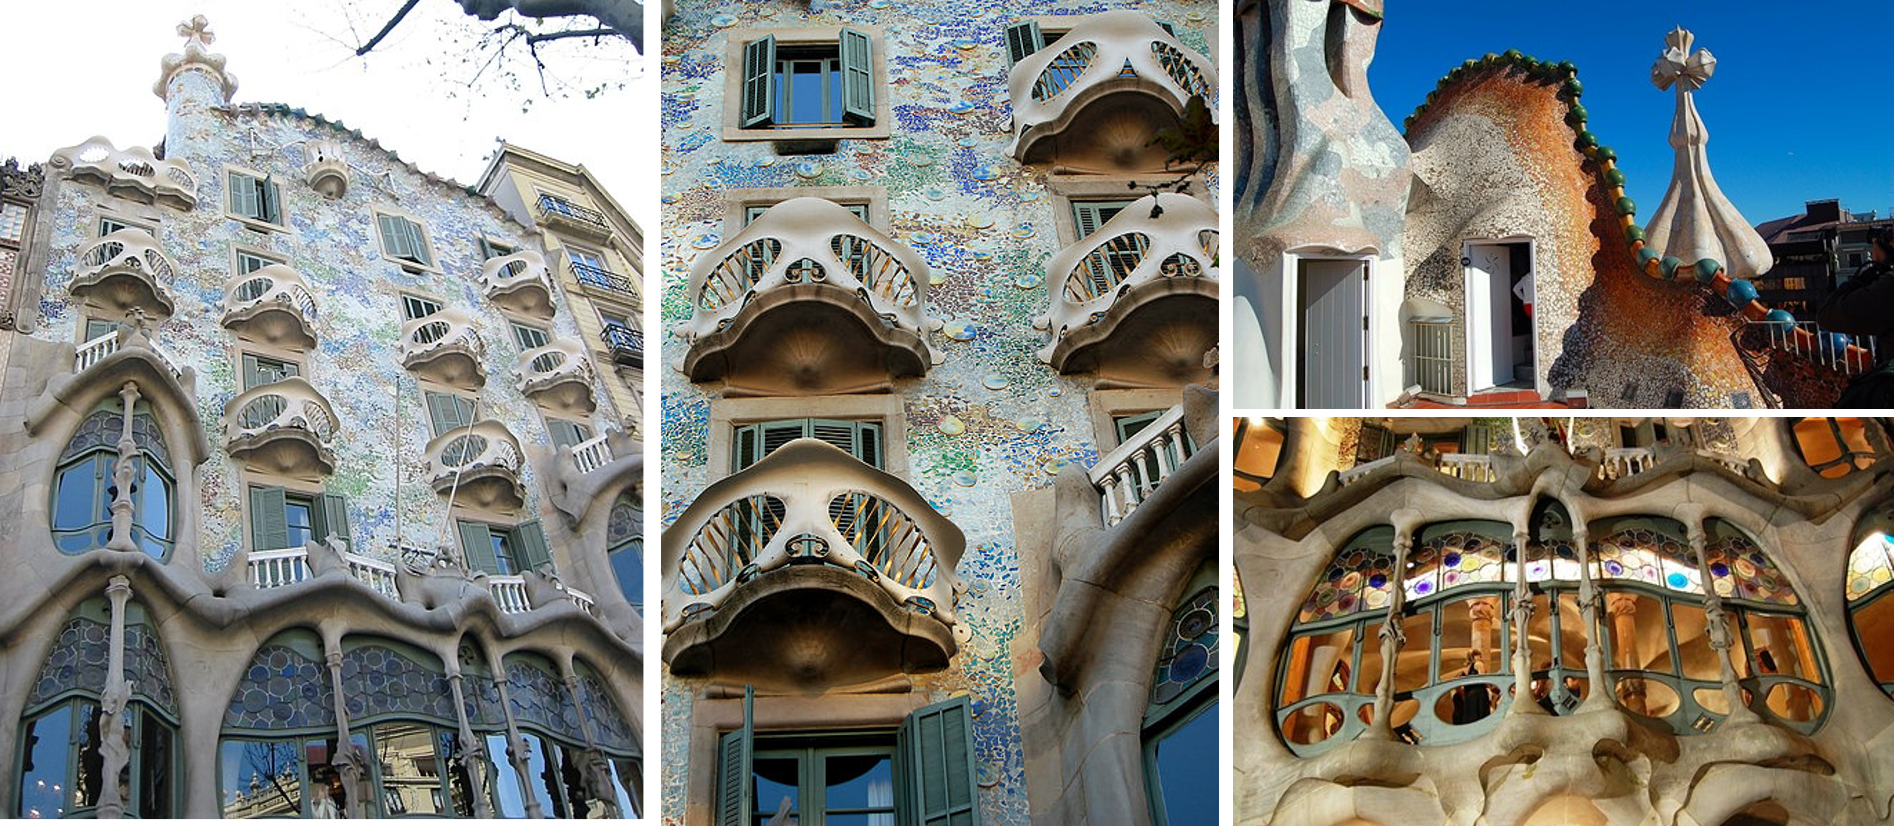
\includegraphics[width= \linewidth]{Images/ArtnouveauGaudi}
          \caption{Facade and ornament according to Art Nouveau style inspired in organic forms, illustrated by Casa Batlló in Barcelona, 1904, designed by Antoni Gaudi. (Left) Casa Batlló's iconic facade. (Middle) A close-up of the intricate mosaic work and balconies. (Upper Right) Ornate mosaic patterns on the roof and (Down Right) windows echoing the textures and colors of the natural world. (\textit{Images edited from source)}}
          \label{fig:ArtNouveaustyle}
        \end{figure}

While the Art Deco style prevalent in Europe and America during in the 1920s to early 1930s will come to rethink Facade and Ornament through the prisms of luxury and technological progress.
This style aimed to capture both modernity and historical nostalgia, resulting in a fusion of futuristic aspirations and references paying homage to the past (Figure\ref{fig:NeoclassicArtDeco}).

%% Figure of Art Deco style  facade
     \begin{figure}[htb]
          \centering
          \includegraphics[width= \linewidth]{Images/ArtDecoFacade}
          \caption{Art Deco Aesthetic of the 1920s to Early 1930s:Art Deco Approach in the 1920s to Early 1930s:  Illustrated by the Chrysler Building, completed in 1930. Facade (Left) and ornamental details (Right) harmonizing futuristic aspirations with references paying homage to the past. (\textit{Images edited from source)}}
          \label{fig:NeoclassicArtDeco}
        \end{figure}

However, while these styles undoubtedly added depth and variety to architectural aesthetics, they did not bring about the same profound paradigm shifts that would later characterize the Modernist movement.

With this broader context established, the analysis will now shift its focus to the Modernist movement's transformative impact on architectural philosophy.

%%facade according to le corbusier

Transitioning from the Baroque style, where facades became expressions of internal dynamics, and acknowledging the enriched insights from the Neoclassical, Art Nouveau and ArtDeco Style,  the historical evolution of facades and ornamentation takes us into the Modernist style of the 20th century—a pivotal juncture that marked one of the most significant shifts in architectural theory.

 Within this era, a radicalized interpretation of ``Form follows function'' emerged, embodying a profound departure from the conventional understanding of facades and ornamentation, partly due to a prevailing stance against ornamentation, often dismissed on moralistic grounds.

Adolf Loos' 1908 article ``Ornament and Crime'' exemplified this sentiment by advocating functional design and condemning conventional ornamentation as unnecessary\cite{Saglam2014}.

Le Corbusier, one of the most prominent figures of this epoch, and renowned for his influential work ``Towards a New Architecture'' first published in 1923, and considered by some to be the most important architectural work published in the 20th century, epitomized the spirit of the era with his distinct views on facades and ornamentation\cite{Studio2a2023}.

Embracing a minimalist and utilitarian approach, Le Corbusier believed that a facade should mirror a building's internal functions, designed in alignment with its purpose and occupants' needs.

Rooted in a human-centric design philosophy, his mantras ``Constructing the architecture of men'' and ``Men are the ones who truly matter'' underscored his commitment to prioritizing people's well-being in his designs\cite{Virseda2021}.

His manifesto ``The Five Points of a New Architecture'' further solidified his design principles.
The notion of ``Free design of the facade'' attained by separating the exterior of the building from its structural function is presented as the means through which the facade liberates itself from conventional structural\cite{Corbusier1986}.

This allowed for the incorporation of large expanses of windows to provide ample natural light and ventilation, fostering a seamless connection between the interior and exterior realms.

Even during this era when ornamentation was viewed unfavorably, Le Corbusier believes in a form of functional ornamentation, as Venturi\cite{Venturi1972} would later accurately point out, Modern architecture uses expressive ornament and shuns explicit symbolic  ornament.

He would ingeniously devise methods to infuse his creations with a distinct form of ornamentation, albeit one rooted in materials' textures, structural elements, and inventive ways of articulating functionality\cite{Saglam2014} that emerged from the building's design.

For example, he used sunshades, brise-soleil, and other shading devices as a way to address climate and control light without compromising the building's aesthetic integrity.

In essence, Le Corbusier's viewpoint on facades and ornamentation epitomized clarity, rationality, and harmonious integration.
His architecture rejected superfluous adornment, and celebrated both technological advancements and structural innovation while maintaining a genuine focus on the well-being and experiences of the occupants (Figure\ref{fig:Modernistfacade}).

%% Figure of Modernist facade and ornament by Le corbusier
     \begin{figure}[htb]
          \centering
          \includegraphics[width= \linewidth]{Images/ModernistFacade}
          \caption{Evolution of Functionalism: Le Corbusier's Journey towards Modernist Facade and Ornamentation. (Left) Villa Savoye, 1928-1931. (Right) Chapelle Notre-Dame-du-Haut de Ronchamp, 1955 (\textit{Images edited from source)}}
          \label{fig:Modernistfacade}
        \end{figure}


%%facade according to Venturi

However, despite the innovative ideals of the Modernist movement,  it became apparent that its utopian vision didn't always materialize as intended.
While the pursuit of functionalism and simplicity was meant to create efficient and logical designs, the outcomes were not always aligned with the intended human experiences.

The Modernist approach often led to the unintentional creation of spaces that felt monotonous and detached from their cultural contexts.
The emphasis on minimalism and the rejection of ornamentation sometimes resulted in environments lacking a sense of identity and character.

The architectural pursuit of universality and timelessness would instead produce sterile, glass-cube structures\cite{Schudel2018} disregarding the importance of cultural heritage and local context, and inadvertently raise the question: Is the reinvention of form, that rejected explicit symbolism and frivolous applique ornament, inspired by the modernist ideals,  yielding a Heroic and original outcome, or is it, instead, a dry expressionism, empty and boring that has distorted the whole building into one big ornament\cite{Venturi1971}.

This scrutiny of the Modernist movement's inability to adequately encompass human experiences and cultural significance, which sparked controversy during the 1960s, brings us to the influential ideas of architect and theorist Robert Venturi.

Venturi's book ``Complexity and Contradiction in Architecture'', published in 1966, marked a turning point in architectural discourse and challenged the prevailing modernist ideals.

Robert Venturi, an iconoclastic architect often hailed as the pioneer of postmodernism\cite{Schudel2018} stood firmly against the oversimplification of architecture, championing the incorporation of contradiction and complexity to yield authentic and vital creations.

The modernist ideals, heavily favoring automobile-centric urban planning, influenced the formation of cities that catered to cars rather than people.
In their thought-provoking book from 1972, "Learning From Las Vegas," Venturi et al.\cite{Venturi1972} put forth a compelling argument, exemplified by the stark contrast seen in places like Las Vegas, they assert that if you were to strip away the dazzling signs, what remains is not a thriving urban environment but a barren desert, illustrating the detachment of architecture relegated to a mere functional necessity camouflaged behind attention-grabbing signs.

Venturi et al.\cite{Venturi1972} will further explain that the oversimplification of architecture, combined with the emergence of sprawling spaces, high speeds, and intricate functions where symbols hold more significance than actual forms, has transformed architecture into symbols occupying space, rather than forming it.

This shift implies that the architectural structure itself carries minimal meaning, with the focus primarily directed towards the signs that communicate with it.

The building stands isolated from the street, often separated by vast parking lots, while the front-facing sign juts out perpendicular to the highway, detached from the building.
At the rear, the structure becomes a utilitarian afterthought, reduced to a budgetary obligation\cite{Venturi1972}.

In this scenario, the absence of signs leaves behind a vacuous atmosphere, characterized by scattered buildings that lack enclosure and cohesion.
The architecture loses its essence, mirroring a cultural void much like a desert devoid of life and enrichment.

The impact of these dynamics is not confined to the past;
instead, they continue to reverberate through the present state of our cities.
Many urban landscapes today still adhere to the principles that emerged from the modernist era.
The prioritization of cars and the resulting sprawling infrastructure persist in shaping cityscapes that often prioritize functionality over human experience.

In response to the challenges posed by the Modernist movement and its unintended consequences, Venturi would reshape the course of architectural discourse.
Notably, he will famously invert the famous dictum of Mies van der Rohe ‘Less is more’ into ‘Less is a bore'\cite{Lutolli2020}, encapsulating his bold departure from the prevailing architectural norms.

In his book ``Complexity and Contradiction in Architecture''\cite{Venturi1977}, Venturi emphasized that architecture should be responsive to the cultural context and the people who inhabit it.

His viewpoint marked a departure from the rigid modernist principles who shunned symbolism of form as an expression or reinforcement of content that dictated that architectural form was to be determined solely by program and structure, with an  occasional  assist from  intuition\cite{Venturi1972}, instead he proposed a reevaluation of the role of ornament and complexity in architectural design (Figure\ref{fig:postmodernfacade}).

%% Figure of Postmodernism facade and ornament
     \begin{figure}[htb]
          \centering
          \includegraphics[width= \linewidth]{Images/PostmodernismVenturi}
          \caption{Postmodernism and the advent of complexity and contradiction (Left) Vanna Venturi House, designed by Robert Venturi and Denise Scott Brown in 1964. (Right) Portland Municipal Services Building, designed by Michael Graves, in 1982 (\textit{Images edited from source)}}
          \label{fig:postmodernfacade}
        \end{figure}

On this context, Venturi believed that a facade could communicate various meanings, evoke emotions, and respond to its cultural and contextual surroundings.
Venturi emphasized the richness of symbolism within architecture, asserting that symbols were fundamental in the architectural language, advocating for the integration of elements from historical precedents and the existing urban fabric, treating them as source materials that could be intelligently referenced or replicated to inform the design process\cite{Venturi1971}.
Importantly, Venturi's approach did not solely prioritize outward appearance;
it was deeply intertwined with the functional aspects of a building's interior, aligning with his belief that architecture should serve both utilitarian purposes and evoke meaningful experiences.

Regarding ornament, he argued that ornamentation was not inherently negative but should be used judiciously and meaningfully.
Venturi coined phrase ``Less is a bore'', suggests his approach towards ornament in what he would describe as ``the decorated shed''\cite{Venturi1972} that architecture doesn't have to be stripped of ornamentation to be considered valid.
He encouraged architects to embrace complexity, contradiction, and the richness of historical references in their designs.

In other words, Robert Venturi's views on facades and ornament emphasized the importance of embracing diversity, historical references, and meaning in architectural design, he wants modern architects to realize only one thing— perfection in the architectural world can and should include imperfection, in all its forms\cite{Lutolli2020}.
This eclectic and innovative design inspired from the return to the ornamentation of the past pushed the boundaries of architecture in the 20th century\cite{Stamp2016}.

In essence, Robert Venturi's perspective on facades and ornamentation underscored the significance of welcoming diversity, historical resonance, and meaningful expression within architectural design.

His vision urged contemporary architects to recognize a crucial reality—perfection within the architectural realm is not confined to flawless forms but also encompasses the beauty found in imperfection, across its myriad manifestations\cite{Lutolli2020}.

This eclectic and innovative approach, which drew inspiration from a renewed appreciation for historical ornamentation, boldly expanded the horizons of architectural exploration throughout the 20th century\cite{Stamp2016} paving the way for the bold explorations and boundary-pushing experiments that would characterize the late 20th century.


=============================
%% Fix the ornamentation and facede descriptions with more concrete examples like do they use geometric lines colors or any specifics
%% prepare the transitioning towards the desconstructivism and revoultion of the late

    %Venturi's stance championed a departure from rigid conformity and highlighted the richness that emerges from embracing the complexities of the human experience and the interconnectedness of design with its cultural, historical, and contextual underpinnings.

%% reorganize the venturi text and seprate it from the critic of modernism. Add a las vegas analyses pic or something related to the soulless architecture. revision the interpretation of facades and ornament with citations before progressing into the contemporary

%%i need to add a paralel that our cities were generated under the modernist ideals and preference of the car which lead to the reference to Las vegas and how if you remove the signs, there is no place only a desert due to the disengage of architecture now reduce to a cheap necessity hidden behind the sign. Also add a picture of the postmodern style with a reference towards facade and ornament made clear in similar fashion as the conclusions of style written before that ussually start with in essence.

%I want to make a reflection at this point, the modernist movement utopia failed and resulted in the creation of monotonous places desensatized from its culture.
%the functionalism was misinterpreted as plainliness and resulted in dehumanized elements.
%the focus on light and glass facades ignored contextual relationship where the climate unapologetically would turn this glass boxes into ovens pradoxical ignoring the maxim of human centric design.
%architecture would follow a pattern regardless of its roots and connection to its local making them virtually indistinguishable from one another in striking contrast to the richful global diversity of the past.
%the absence of ornament was misinterpreted as the lack of effort reducing architecture to mere construction.

   %%%==========================References




    \subsection{Quantitative Image complexity Analysis}
    \label{subsec:ComplexityImageAnalysis}
    %!\subsection{Quantitative complexity Analysis}
%    \label{subsec:ComplexityImageAnalysis}
%    %!\subsection{Quantitative complexity Analysis}
%    \label{subsec:ComplexityImageAnalysis}
%    %!\subsection{Quantitative complexity Analysis}
%    \label{subsec:ComplexityImageAnalysis}
%    \input{Text/ComplexityImageAnalysis.tex}

We have previously discussed the argument that the architectural evolution, throughout history, has been characterized by a continual interplay between simplicity and complexity.
This notion has been substantiated by our exploration of the theoretical definitions and varied approaches to facades and ornamentation within the context of prominent architectural styles and the perspectives of their eminent architects.

Our literature review has consistently pointed towards a prevailing trend in contemporary architecture, suggesting a resurgence of complexity in architectural design.
However, to ensure our findings are not purely subjective or biased towards this conclusion, we have conducted a quantitative analysis using Image Complexity Analysis.
This rigorous analysis method utilizes input images of the most iconic and representative buildings from various epochs and styles.

Through Image Complexity Analysis, we assign a quantitative complexity value to these architectural images.
This complexity value is derived from a comprehensive examination of spatial intricacies, frequency patterns, and color information present within, based on the research strategy by Ishra et al\cite{Ishrat2020}.

By employing this quantitative approach, we aim to provide an objective measure of the shift from simplicity towards complexity in architecture, further strengthening the thesis of an impending era characterized by architectural intricacy and richness in facades and ornamentation.

The results are visually depicted in Figure\ref{fig:complexitygraph}, where a discernible upward trendline emerges, particularly noticeable since the late 20th century.
This graphical representation unmistakably illustrates a growing inclination towards architecturally complex designs, further corroborating the conclusion drawn from our extensive literature review.

%% Figure of Complexity graph
     \begin{figure*}[htb]
          \centering
          \includegraphics[width= \linewidth]{Graphs/complexitygraph}
          \caption{Contemporary architecture. An era of exploration. (from left to right) Desconstructivism, Neofuturism, High-tech modernism, Parametricism, Pragmatic utopinaism.  (\textit{Images edited from source)}}
          \label{fig:complexitygraph}
        \end{figure*}


=========

 Complexity of an image is governed by spatial, frequency and color information present in the image.\cite{Ishrat2020}

Scanpath based image complexity analysis determines human visual behavior that could lead to development of interactive and intelligent systems.\cite{Ishrat2020}

The objective of current research work is to establish the complexity of the given set of images while target objects are searched and to present analysis ofgaze search pattern.
To achieve these objectives a remote gaze estimation and analysis model has been proposed for scanpath identification and analysis.\cite{Ishrat2020}






We have previously discussed the argument that the architectural evolution, throughout history, has been characterized by a continual interplay between simplicity and complexity.
This notion has been substantiated by our exploration of the theoretical definitions and varied approaches to facades and ornamentation within the context of prominent architectural styles and the perspectives of their eminent architects.

Our literature review has consistently pointed towards a prevailing trend in contemporary architecture, suggesting a resurgence of complexity in architectural design.
However, to ensure our findings are not purely subjective or biased towards this conclusion, we have conducted a quantitative analysis using Image Complexity Analysis.
This rigorous analysis method utilizes input images of the most iconic and representative buildings from various epochs and styles.

Through Image Complexity Analysis, we assign a quantitative complexity value to these architectural images.
This complexity value is derived from a comprehensive examination of spatial intricacies, frequency patterns, and color information present within, based on the research strategy by Ishra et al\cite{Ishrat2020}.

By employing this quantitative approach, we aim to provide an objective measure of the shift from simplicity towards complexity in architecture, further strengthening the thesis of an impending era characterized by architectural intricacy and richness in facades and ornamentation.

The results are visually depicted in Figure\ref{fig:complexitygraph}, where a discernible upward trendline emerges, particularly noticeable since the late 20th century.
This graphical representation unmistakably illustrates a growing inclination towards architecturally complex designs, further corroborating the conclusion drawn from our extensive literature review.

%% Figure of Complexity graph
     \begin{figure*}[htb]
          \centering
          \includegraphics[width= \linewidth]{Graphs/complexitygraph}
          \caption{Contemporary architecture. An era of exploration. (from left to right) Desconstructivism, Neofuturism, High-tech modernism, Parametricism, Pragmatic utopinaism.  (\textit{Images edited from source)}}
          \label{fig:complexitygraph}
        \end{figure*}


=========

 Complexity of an image is governed by spatial, frequency and color information present in the image.\cite{Ishrat2020}

Scanpath based image complexity analysis determines human visual behavior that could lead to development of interactive and intelligent systems.\cite{Ishrat2020}

The objective of current research work is to establish the complexity of the given set of images while target objects are searched and to present analysis ofgaze search pattern.
To achieve these objectives a remote gaze estimation and analysis model has been proposed for scanpath identification and analysis.\cite{Ishrat2020}






We have previously discussed the argument that the architectural evolution, throughout history, has been characterized by a continual interplay between simplicity and complexity.
This notion has been substantiated by our exploration of the theoretical definitions and varied approaches to facades and ornamentation within the context of prominent architectural styles and the perspectives of their eminent architects.

Our literature review has consistently pointed towards a prevailing trend in contemporary architecture, suggesting a resurgence of complexity in architectural design.
However, to ensure our findings are not purely subjective or biased towards this conclusion, we have conducted a quantitative analysis using Image Complexity Analysis.
This rigorous analysis method utilizes input images of the most iconic and representative buildings from various epochs and styles.

Through Image Complexity Analysis, we assign a quantitative complexity value to these architectural images.
This complexity value is derived from a comprehensive examination of spatial intricacies, frequency patterns, and color information present within, based on the research strategy by Ishra et al\cite{Ishrat2020}.

By employing this quantitative approach, we aim to provide an objective measure of the shift from simplicity towards complexity in architecture, further strengthening the thesis of an impending era characterized by architectural intricacy and richness in facades and ornamentation.

The results are visually depicted in Figure\ref{fig:complexitygraph}, where a discernible upward trendline emerges, particularly noticeable since the late 20th century.
This graphical representation unmistakably illustrates a growing inclination towards architecturally complex designs, further corroborating the conclusion drawn from our extensive literature review.

%% Figure of Complexity graph
     \begin{figure*}[htb]
          \centering
          \includegraphics[width= \linewidth]{Graphs/complexitygraph}
          \caption{Contemporary architecture. An era of exploration. (from left to right) Desconstructivism, Neofuturism, High-tech modernism, Parametricism, Pragmatic utopinaism.  (\textit{Images edited from source)}}
          \label{fig:complexitygraph}
        \end{figure*}


=========

 Complexity of an image is governed by spatial, frequency and color information present in the image.\cite{Ishrat2020}

Scanpath based image complexity analysis determines human visual behavior that could lead to development of interactive and intelligent systems.\cite{Ishrat2020}

The objective of current research work is to establish the complexity of the given set of images while target objects are searched and to present analysis ofgaze search pattern.
To achieve these objectives a remote gaze estimation and analysis model has been proposed for scanpath identification and analysis.\cite{Ishrat2020}






    \subsection{Digital fabrication and Environmental Sustainability}
    \label{subsec:DigitalFabricationAndEnvSustainability}
    
%!\subsection{Digital fabrication and Environmental Sustainability}
%!\label{subsec:DigitalFabricationAndEnvSustainability}

%!==========================
%8. **Environmental Sustainability:** Investigate how the integration of complex facades and digital fabrication aligns with contemporary sustainability principles. Examine how parametric design and data-driven approaches can enhance energy efficiency, reduce material waste, and contribute to sustainable construction practices.
%!==========================
To be revised ...
%!original

%Digital fabrication technologies, meanwhile, are interacting with the biological world on a daily basis.
%Engineers, designers, and architects are combining computational design, additive manufacturing, materials engineering, and synthetic biology to pioneer a symbiosis between microorganisms, our bodies, the products we consume, and even the buildings we inhabit\cite{Schwab2016}.







    \subsection{Future Trends and speculations}
    \label{subsec:Futuretrends}
    %!\subsection{Future Trends and speculations}
%!\label{subsec:Futuretrends}

%!==========================
%Speculate on the potential future trajectories of architectural design, digital fabrication, and mixed reality. Discuss how these trends might shape the built environment, and propose ideas for further research and exploration.
%!==========================

%!\subsection{Object-Oriented Ontology}
%!\label{subsec:ObjectOrientedOntology}
% add the concept of Object-Oriented. Using these concepts as basis. I want to express that the mr experiment is based on the idea that architecture as a tool should be invisible and confortable while in use. But it should  create emotion when seen as part of the landscape as a form of art to recapture the humand oriented city .

It may be cheaper and quicker to build a load-bearing brick wall, but
the High Tech architect will always prefer the steel frame and the lightweight metal panel because this is a technique more in tune with the spirit of the age.
He is committed to the idea that building must eventually catch up with the rest of technology, and he is determined to "drag building into the twentieth century".\cite{Davies1988}

Heideggers tool analysis states that as the tool is a tool it disappears in favor of some purpose he continues to explain that generally we don't notice equipment until it fails, like when An earthquake calls attention to the ground we walk or when a medical problem alerts us of the presence of organs that we have silently depended\cite{Harman2011}.
Harmans, Object-oriented ontology, borrows this concept to formulate its central claim that objects have hidden qualities and realities, and they withdraw from our understanding.\cite{Gage2015}
he idea that we live our lives on a layer of invisible equipment has significant ramifications for architecture, a discipline that produces the equipment on and in which we exist.\cite{Gage2015}

(Figure \ref{fig:complexornament})

%% Figure of Contemporary timeline
     \begin{figure*}[htb]
          \centering
          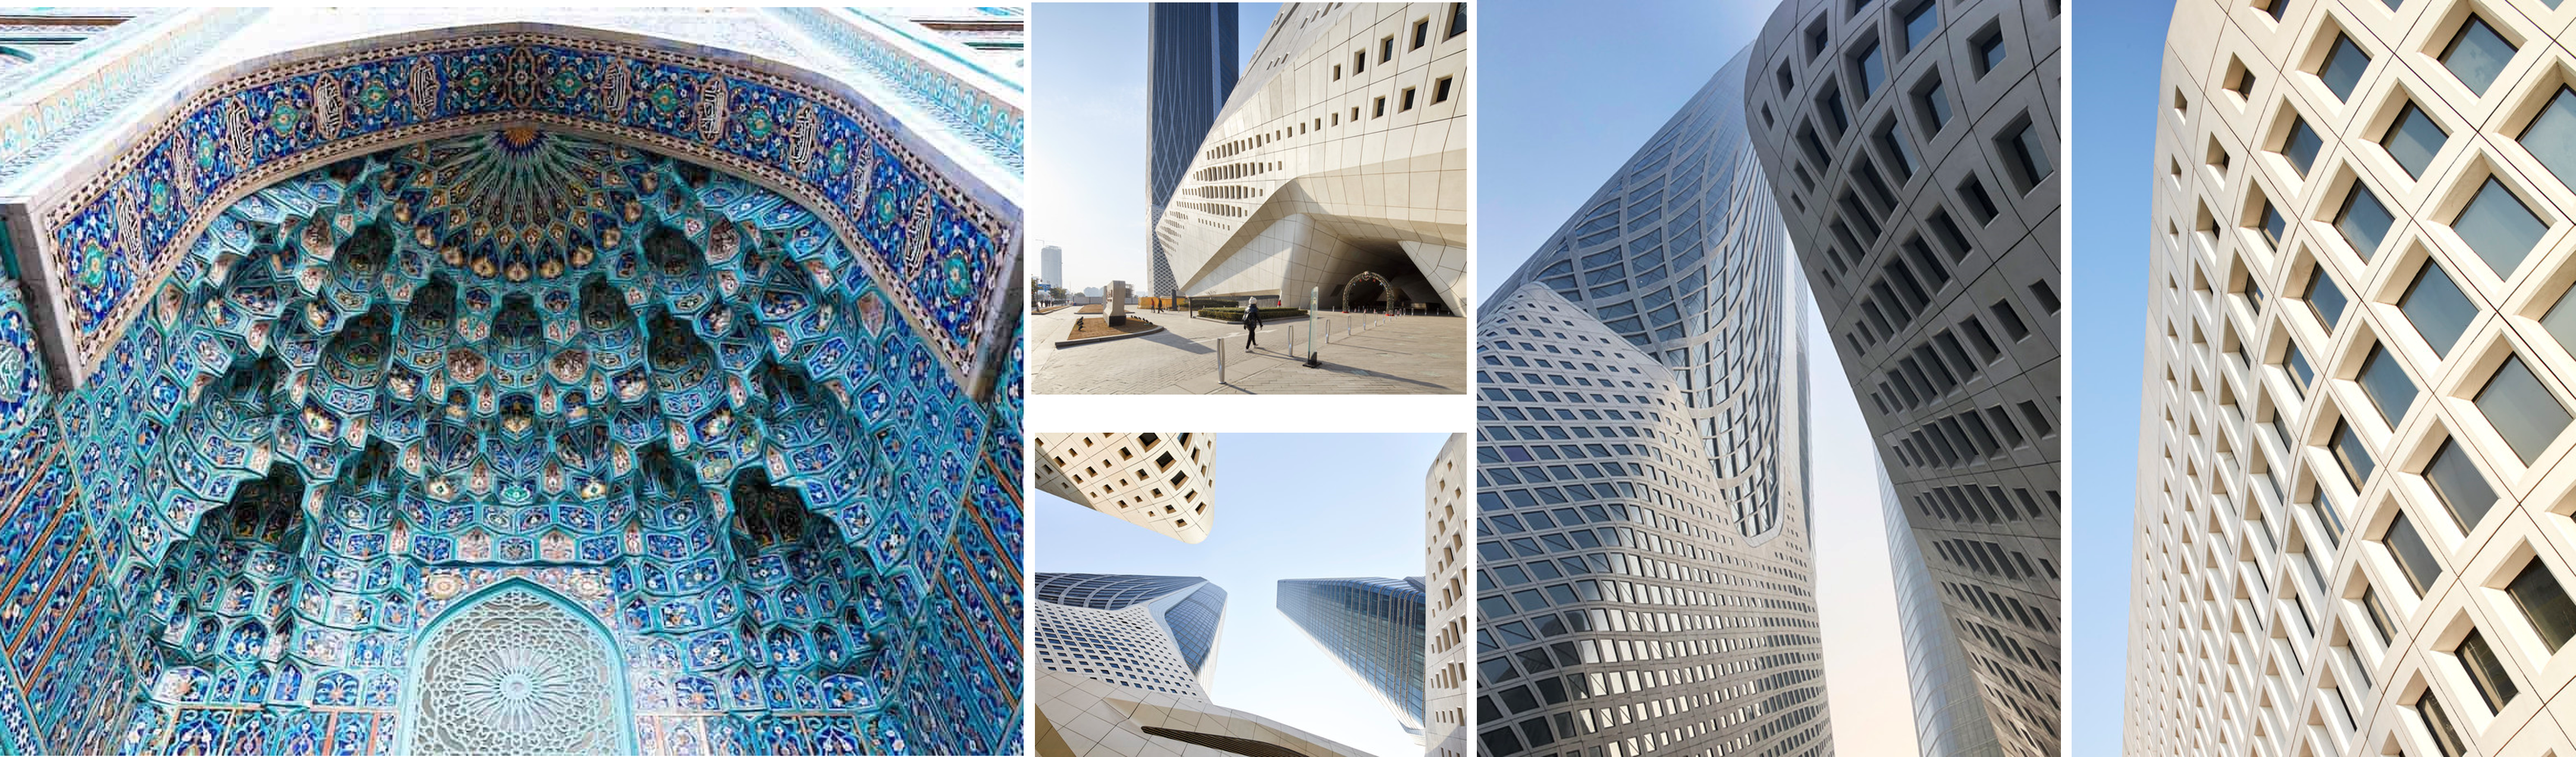
\includegraphics[width= \linewidth]{Images/complexornament}
          \caption{Complex ornament reference  (\textit{Images edited from source)}}
          \label{fig:complexornament}
        \end{figure*}


\section{Methodology}
\label{sec:Methodology}
%%Methodology
%% methodology Intro
The methodology of this study, comprises three main components (as illustrated in  Figure~\ref{fig:MethodologyFlowchart}):

\begin{itemize}
    \item Computational Image Complexity Analysis (CICA) system
    \item VR System Development
    \item Experiment Design
\end{itemize}

\textbf{CICA system:} Detailed in Section~\ref{subsec:Computational Image Complexity analysis} and depicted as (3.1) in Figure~\ref{fig:MethodologyFlowchart}, involves developing a Python script using computer vision algorithms to process images and yield complexity scores, quantitatively gauging the intricacy of architectural designs.
It supports theoretical analyses and provides a ranking framework for facade designs in the VR system.

\textbf{VR System Development:}  Outlined in Section~\ref{subsec:VRsystemDevelopment} and represented as (3.2) in Figure~\ref{fig:MethodologyFlowchart}, this component focuses on creating an immersive experience where participants can explore and interact with a building's interior and exterior, manipulating facade designs with variable complexity levels and experiencing their impact.

\textbf{Experiment Design:} Detailed in Section~\ref{subsec:Experiment_design} and illustrated as (3.3) in Figure~\ref{fig:MethodologyFlowchart}, following a similar approach to previous studies~\cite{Wolfartsberger2019}, this component outlines the method to evaluate users' acceptance of building complexity.
It consists of three stages: a VR interaction stage, a screen-based stage, and a post-interaction survey.
These stages allow for the collection of quantitative and qualitative data on participants' perceptions and responses to different complexity levels in facade designs.

As illustrated in the methodology flowchart (Figure~\ref{fig:MethodologyFlowchart}), these components are combined to integrate computational analysis with immersive VR experiments, exploring user preferences in facade design and providing insights into architectural trends.

With this methodology outlined, the following sections will now delve into a comprehensive breakdown of each component, highlighting their objectives, methodologies, and significance in achieving our research goals.




\section{Results}
\label{sec:Results}
%% Results should be clear and concise.
%\section{Results}
%\label{sec:Results}
%% Results should be clear and concise.

The experiment to test the hypothesis that participants in virtual reality (VR) experiments would be more likely to favor data-driven design recommendations for Site Layout Planning (SLP) design was conducted at the Kyushu University campus in Fukuoka, Japan, over a period of 15 days, from June 10 to 25, 2023, during the afternoon hours between 13:00 and 18:00.

A total of 17 participants took part in the experiment, primarily consisting of university students and faculty members. The participants had diverse professional backgrounds, as shown in Figure \ref{fig:ParticipantBackgroundChart}, with over \(50\%\) being students from various faculties, approximately \(20\%\) having a construction background, and \(23.5\%\) reporting previous experience in SLP, as indicated in Figure \ref{fig:YearsExperienceChart}

    %% Participant background chart and years of experience
    \begin{table*}[htb]
        \centering
        \small
        \begin{tabularx}{\textwidth}{X X}
            \centering
            % trim=left 190 down 250 right 150 top5
            \includegraphics[width=\linewidth, trim=0 50 0 50]{Images/ParticipantBackgroundChart.pdf}
            \captionof{figure}{Professional Background of participants in the experiment for VR in SLP}
            \label{fig:ParticipantBackgroundChart} &
            \centering
            \includegraphics[width=\linewidth, trim=0 50 0 50]{Images/YearsExperienceChart.pdf}
            \captionof{figure}{Years of experience in SLP of participants in the experiment for VR in SLP}
            \label{fig:YearsExperienceChart}
        \end{tabularx}
    \end{table*}

Regarding the first metric, accuracy analysis, most participants completed the SLP task for all three sites, resulting in a total of 39 experiment sessions. For each site, two outcomes were recorded: the position selected during the "screen-based interaction" stage and the "VR interaction" stage. These outcomes were summarized in radial graphs, referred to as "accuracy analysis graphs," as depicted in Figure \ref{fig:Accuracyscattergraph}.

     %% Figure Accuracy graph
        \begin{figure*}[htb]
          \centering
          \includegraphics[width= \linewidth, trim=0 0 0 0]{Images/ComplexityPerceptionPerLevel}
          \caption{Complexity perception graph per level of complexity defined for each of the 10 variations generated for each of the three patterns compared to the original ranking. Illustration of the deviation between the complexity perceived by the participants and the original ranking during the screen-based stage of the experiment.}
          \label{fig:ComplexityPerceptionPerLevel}
        \end{figure*}

In these graphs, the center serves as a reference point, representing the top recommendation provided by the optimization system for each specific site. The coordinates of this center point vary for each site, reflecting the distinct optimal locations suggested by the system. On the other hand, the participants' chosen locations are plotted on the graph, precisely indicating the positions they deemed most suitable for the new educational building within the boundaries of the site.

The placement of each participant's chosen location on the graph is based on its actual geographical coordinates, ensuring an accurate representation of their decision-making process. The distance between each participant's chosen location and the center reflects the deviation error from the system's top recommendation, allowing for a clear assessment of how closely participants' choices align with the data-driven optimization results.

Furthermore, the orientation of each chosen location on the graph provides valuable insights into the direction in which participants opted to position the building, allowing for a comprehensive understanding of their decision-making rationale. Overall, these accuracy analysis graphs present an actual representation of the chosen locations on the physical site, capturing both spatial proximity and directional preferences relative to the system's top recommendation.

The purpose of the analysis was to evaluate the reduction in the deviation error between the preferred SLP location recommended by our Multi-objective optimization (MOO) model and the location ultimately chosen by the experiment participants in both the "screen-based" and "VR interaction" stages of the experiment.

By analyzing the accuracy analysis graphs, the contribution of the VR system was determined by examining the vector resultant from the center point (top recommendation) to the participant's chosen location. A reduction in the vector magnitude in the "VR answer" compared to the "screen-based answer" indicated an improvement percentage, while an increase represented a decline. This analysis allowed us to quantify the impact of VR immersion on participants' decision-making accuracy in SLP design.

The accuracy analysis results, depicted in the "Accuracy improvement" bar chart in Figure \ref{fig:ImprovementChart}, showcased varying degrees of improvement among the 39 experiment sessions, with only three cases showing a decline. On average, there was a \(48.3\%\) improvement among the participants.

The accuracy analysis results, illustrated in the "Accuracy improvement" bar chart (Figure \ref{fig:ImprovementChart}), revealed varying degrees of improvement among the 39 experiment sessions, with only three cases showing a decline. On average, there was a significant \(48.3\%\) improvement among the participants.



    % Complexity level chosen Chart
    \begin{figure}[htb]
        \centering
        %trim=100 180 100 120, clip
        \includegraphics[width=\linewidth]{Images/ComplexityLevelChosenChart}
        \caption{Complexity level chosen among participants during the VR simulation for all three patterns}
        \label{fig:ComplexityLevelChosenChart}
    \end{figure}


    % Complexity perception Chart
    \begin{figure}[htb]
        \centering
        %trim=100 180 100 120, clip
        \includegraphics[width=\linewidth]{Images/ComplexityPerceptionChart}
        \caption{Improvement in accuracy among participants with the use of VR simulation compared to the screen-based simulation}
        \label{fig:ComplexityPerceptionChart}
    \end{figure}

The accuracy improvement percentage results exhibited a wide distribution, as indicated by the current standard deviation of \(44.1\%\).
The probability bell graph displayed in Figure \ref{fig:ProbabilityScatterGraph} further illustrated the significant variability in the results, emphasizing the uncertainty in predicting individual data points or outcomes.


% probability preferred complexity level Chart
    \begin{figure}[htb]
        \centering
        \includegraphics[width=\linewidth]{Images/ProbabilityPreferredComplexitylevel}
        \caption{Probability of preferred complexity level for facade design}
        \label{fig:ProbabilityComplexitylevelChart}
    \end{figure}

Analyzing the average improvement in accuracy per site (Figure \ref{fig:ImprovementPerSite}) revealed a potential correlation between the level of improvement and the complexity of a site's topography.
This finding suggests that VR-based approaches may have a stronger positive impact on decision-making when dealing with more intricate and challenging terrains.

     % Improvement per Site Chart and Performance indicator Weight
    \begin{table*}[htb]
        \centering
        \small
        \begin{tabularx}{\textwidth}{X X}
            \centering
            \includegraphics[width=\linewidth, trim=0 0 0 20]{Images/PerformanceIndicatorWeightChart}
            \captionof{figure}{Average of weight distribution when ranking importance of the performance indicators, defined by the participants, per site.}
            \label{fig:PerformanceIndicatorweightChart} &
            \centering
            \includegraphics[width=\linewidth, trim=0 0 0 20]{Images/PreferredComplexityLevelPerPattern}
            \captionof{figure}{Average of preferred complexity level per pattern during the VR simulation, with detail of the overall average of the experiment (Mean = \(48.3\%\))}
            \label{fig:ImprovementPerSite}
        \end{tabularx}
    \end{table*}

The survey results provided additional insights into the influence of VR interaction and data-driven optimization for SLP. The ``influence perception'' section of the survey, depicted in Figure\ref{fig:PerceptionSatisfactionSurveyResults}, indicated that the system scored above 5 on a 7-point Likert scale for all questions, suggesting a positive influence of the VR strategy in introducing data-driven recommendations. This finding aligned with the accuracy improvement percentage results observed in the accuracy analysis (Figure\ref{fig:ImprovementChart}).

    %% Perception Satisfaction Survey and Usability results
    \begin{table*}[htb]
        \centering
        \small
        \begin{tabularx}{\textwidth}{X X}
            \centering
            \includegraphics[width=\linewidth]{Images/UsabilityChartSurvey}
            \captionof{figure}{"User Satisfaction section questions from User Survey of SLP System. \- (n = 17), 1 - strongly disagree, 7 - strongly agree}
            \label{fig:UsabilityChartSurvey} &
            \centering
            \includegraphics[width=\linewidth]{Images/PerceptionChartSurvey}
            \captionof{figure}{User-System Influence Perception section" questions. \- (n = 17), 1 - strongly disagree, 7 - strongly agree}
            \label{fig:PerceptionSatisfactionSurveyResults}
        \end{tabularx}
    \end{table*}

During post-experiment interviews, participants were asked for their opinions on the weight distribution used by the optimization model to balance the trade-offs between the three performance indicators. The initial distribution decided for the system was set at 50, 30, and 20 for the respective indicators (see Table \ref{tab:PerformanceIndicators}). While most participants maintained a consistent criteria for ranking the indicators, slight deviations from the predetermined weight distribution were observed. Figure \ref{fig:PerformanceIndicatorweightChart} visually represents the average weight configuration suggested by the participants, demonstrating their individual preferences in adjusting the trade-off weights for each site.

Overall, the results support the initial hypothesis, indicating that VR has the potential to enhance the acceptance of data-driven design recommendations in SLP. However, the "user satisfaction" section of the survey, summarized in Figure \ref{fig:UsabilityChartSurvey}, revealed room for improvement in the user interface and experience, with scores above 4.5 on a 7-point Likert scale. Notably, the areas of helpfulness and visualization enhancement ranked the lowest, despite initially being considered key advantages of the "VR interaction" system compared to the "screen-based" alternative.



\section{Discussion}
\label{sec:Discussion}
%% This should explore the significance of the results of the work, not repeat them. A combined Results and Discussion section is often appropriate. Avoid extensive citations and discussion of published literature.
%%!\section{Discussion}
%\label{sec:Discussion}
%%% This should explore the significance of the results of the work, not repeat them. A combined Results and Discussion section is often appropriate. Avoid extensive citations and discussion of published literature.
%%%!\section{Discussion}
%\label{sec:Discussion}
%%% This should explore the significance of the results of the work, not repeat them. A combined Results and Discussion section is often appropriate. Avoid extensive citations and discussion of published literature.
%%%!\section{Discussion}
%\label{sec:Discussion}
%%% This should explore the significance of the results of the work, not repeat them. A combined Results and Discussion section is often appropriate. Avoid extensive citations and discussion of published literature.
%%\input{Text/Discussion}

Discussion on results of history analysis and how theory aligns with the computational image analysis.
Followed by a tuning of the level of complexity how we interpret the survey results to propose a graphical conclusion of an apparent complex facade inside the boundaries of tolerance given by the experiment participants.

%! Historical Analysis graph

Through Image Complexity Analysis, we assign a quantitative complexity value to these architectural images.
This complexity value is derived from a comprehensive examination of spatial intricacies, frequency patterns, and color information present within, based on the research strategy by Ishra et al\cite{Ishrat2020}.

By employing this quantitative approach, we aim to provide an objective measure of the shift from simplicity towards complexity in architecture, further strengthening the thesis of an impending era characterized by architectural intricacy and richness in facades and ornamentation.

This graphical representation unmistakably illustrates a growing inclination towards architecturally complex designs, further corroborating the conclusion drawn from our extensive literature review.
%=========
%
% Complexity of an image is governed by spatial, frequency and color information present in the image.\cite{Ishrat2020}
%
%Scanpath based image complexity analysis determines human visual behavior that could lead to development of interactive and intelligent systems.\cite{Ishrat2020}
%
%The objective of current research work is to establish the complexity of the given set of images while target objects are searched and to present analysis ofgaze search pattern.
%To achieve these objectives a remote gaze estimation and analysis model has been proposed for scanpath identification and analysis.\cite{Ishrat2020}


%! Experiment results discussions


Discussion on results of history analysis and how theory aligns with the computational image analysis.
Followed by a tuning of the level of complexity how we interpret the survey results to propose a graphical conclusion of an apparent complex facade inside the boundaries of tolerance given by the experiment participants.

%! Historical Analysis graph

Through Image Complexity Analysis, we assign a quantitative complexity value to these architectural images.
This complexity value is derived from a comprehensive examination of spatial intricacies, frequency patterns, and color information present within, based on the research strategy by Ishra et al\cite{Ishrat2020}.

By employing this quantitative approach, we aim to provide an objective measure of the shift from simplicity towards complexity in architecture, further strengthening the thesis of an impending era characterized by architectural intricacy and richness in facades and ornamentation.

This graphical representation unmistakably illustrates a growing inclination towards architecturally complex designs, further corroborating the conclusion drawn from our extensive literature review.
%=========
%
% Complexity of an image is governed by spatial, frequency and color information present in the image.\cite{Ishrat2020}
%
%Scanpath based image complexity analysis determines human visual behavior that could lead to development of interactive and intelligent systems.\cite{Ishrat2020}
%
%The objective of current research work is to establish the complexity of the given set of images while target objects are searched and to present analysis ofgaze search pattern.
%To achieve these objectives a remote gaze estimation and analysis model has been proposed for scanpath identification and analysis.\cite{Ishrat2020}


%! Experiment results discussions


Discussion on results of history analysis and how theory aligns with the computational image analysis.
Followed by a tuning of the level of complexity how we interpret the survey results to propose a graphical conclusion of an apparent complex facade inside the boundaries of tolerance given by the experiment participants.

%! Historical Analysis graph

Through Image Complexity Analysis, we assign a quantitative complexity value to these architectural images.
This complexity value is derived from a comprehensive examination of spatial intricacies, frequency patterns, and color information present within, based on the research strategy by Ishra et al\cite{Ishrat2020}.

By employing this quantitative approach, we aim to provide an objective measure of the shift from simplicity towards complexity in architecture, further strengthening the thesis of an impending era characterized by architectural intricacy and richness in facades and ornamentation.

This graphical representation unmistakably illustrates a growing inclination towards architecturally complex designs, further corroborating the conclusion drawn from our extensive literature review.
%=========
%
% Complexity of an image is governed by spatial, frequency and color information present in the image.\cite{Ishrat2020}
%
%Scanpath based image complexity analysis determines human visual behavior that could lead to development of interactive and intelligent systems.\cite{Ishrat2020}
%
%The objective of current research work is to establish the complexity of the given set of images while target objects are searched and to present analysis ofgaze search pattern.
%To achieve these objectives a remote gaze estimation and analysis model has been proposed for scanpath identification and analysis.\cite{Ishrat2020}


%! Experiment results discussions



\section{Conclusions}
\label{sec:Conclusion}
%% The main conclusions of the study may be presented in a short Conclusions section, which may stand alone or form a subsection of a Discussion or Results and Discussion section.
%%!%\section{Conclusions}
%%\label{sec:Conclusion}
%%%!%\section{Conclusions}
%%\label{sec:Conclusion}
%%%!%\section{Conclusions}
%%\label{sec:Conclusion}
%%\input{Text/Conclusions}

%% The main conclusions of the study may be presented in a short Conclusions section, which may stand alone or form a subsection of a Discussion or Results and Discussion section.
%% Answer the Research question

%revision

This research investigates architectural design at the intersection of digital fabrication, virtual reality (VR) assessment, and computer vision, aiming to deepen our understanding of complexity in facade design.
Our primary goal is to gauge user tolerance and acceptance of complex facades, offering insights into future construction practices.

A literature review confirmed that contemporary architecture is witnessing a trend towards increasing complexity in facade designs, moving away from the minimalist approach of the modernist movement, a trend also evidenced by the quantitative analysis across architectural history, provided by the `Computational Image Complexity Analysis' (CICA) system, which revealed an upward complexity trendline since the late 20th century (see Figure~\ref{fig:CICAscatterGraphRender}).
The historical analysis using the CICA system underscored the cultural and historical significance of facades, indicating that architectural complexity is not merely a matter of quantitative metrics but also involves cultural resonance and historical context.

Participants in the virtual reality experiment showed a preference for facades with moderate complexity, suggesting that future architectural trends may favor designs that balance intricacy with simplicity.
On average, participants favor a moderate level of complexity, with an average CICA complexity score of 3.82 (out of 10) and a 40\% probability of selecting a score close to this value according to CICA\@.

Discrepancies between participant perceptions and the CICA system's complexity rankings were particularly evident at higher complexity levels.
This highlights the subjective nature of complexity perception and the importance of integrating human feedback into architectural assessments.

The qualitative data suggests a shift towards customizable and user-responsive architectural solutions, with participants favoring form over materials and expressing a preference for facades that consider views and privacy.
This feedback suggests a strategic, view-dependent approach to facade complexity is crucial for user satisfaction.

In conclusion, this study underscores a shift in contemporary architecture towards embracing complexity in facade design, moving beyond the minimalist constraints of the modernist movement.
These insights could inform the development of nuanced and user-centric approaches in architectural design, catering to the evolving demands of modern society.


%% The main conclusions of the study may be presented in a short Conclusions section, which may stand alone or form a subsection of a Discussion or Results and Discussion section.
%% Answer the Research question

%revision

This research investigates architectural design at the intersection of digital fabrication, virtual reality (VR) assessment, and computer vision, aiming to deepen our understanding of complexity in facade design.
Our primary goal is to gauge user tolerance and acceptance of complex facades, offering insights into future construction practices.

A literature review confirmed that contemporary architecture is witnessing a trend towards increasing complexity in facade designs, moving away from the minimalist approach of the modernist movement, a trend also evidenced by the quantitative analysis across architectural history, provided by the `Computational Image Complexity Analysis' (CICA) system, which revealed an upward complexity trendline since the late 20th century (see Figure~\ref{fig:CICAscatterGraphRender}).
The historical analysis using the CICA system underscored the cultural and historical significance of facades, indicating that architectural complexity is not merely a matter of quantitative metrics but also involves cultural resonance and historical context.

Participants in the virtual reality experiment showed a preference for facades with moderate complexity, suggesting that future architectural trends may favor designs that balance intricacy with simplicity.
On average, participants favor a moderate level of complexity, with an average CICA complexity score of 3.82 (out of 10) and a 40\% probability of selecting a score close to this value according to CICA\@.

Discrepancies between participant perceptions and the CICA system's complexity rankings were particularly evident at higher complexity levels.
This highlights the subjective nature of complexity perception and the importance of integrating human feedback into architectural assessments.

The qualitative data suggests a shift towards customizable and user-responsive architectural solutions, with participants favoring form over materials and expressing a preference for facades that consider views and privacy.
This feedback suggests a strategic, view-dependent approach to facade complexity is crucial for user satisfaction.

In conclusion, this study underscores a shift in contemporary architecture towards embracing complexity in facade design, moving beyond the minimalist constraints of the modernist movement.
These insights could inform the development of nuanced and user-centric approaches in architectural design, catering to the evolving demands of modern society.


%% The main conclusions of the study may be presented in a short Conclusions section, which may stand alone or form a subsection of a Discussion or Results and Discussion section.
%% Answer the Research question

%revision

This research investigates architectural design at the intersection of digital fabrication, virtual reality (VR) assessment, and computer vision, aiming to deepen our understanding of complexity in facade design.
Our primary goal is to gauge user tolerance and acceptance of complex facades, offering insights into future construction practices.

A literature review confirmed that contemporary architecture is witnessing a trend towards increasing complexity in facade designs, moving away from the minimalist approach of the modernist movement, a trend also evidenced by the quantitative analysis across architectural history, provided by the `Computational Image Complexity Analysis' (CICA) system, which revealed an upward complexity trendline since the late 20th century (see Figure~\ref{fig:CICAscatterGraphRender}).
The historical analysis using the CICA system underscored the cultural and historical significance of facades, indicating that architectural complexity is not merely a matter of quantitative metrics but also involves cultural resonance and historical context.

Participants in the virtual reality experiment showed a preference for facades with moderate complexity, suggesting that future architectural trends may favor designs that balance intricacy with simplicity.
On average, participants favor a moderate level of complexity, with an average CICA complexity score of 3.82 (out of 10) and a 40\% probability of selecting a score close to this value according to CICA\@.

Discrepancies between participant perceptions and the CICA system's complexity rankings were particularly evident at higher complexity levels.
This highlights the subjective nature of complexity perception and the importance of integrating human feedback into architectural assessments.

The qualitative data suggests a shift towards customizable and user-responsive architectural solutions, with participants favoring form over materials and expressing a preference for facades that consider views and privacy.
This feedback suggests a strategic, view-dependent approach to facade complexity is crucial for user satisfaction.

In conclusion, this study underscores a shift in contemporary architecture towards embracing complexity in facade design, moving beyond the minimalist constraints of the modernist movement.
These insights could inform the development of nuanced and user-centric approaches in architectural design, catering to the evolving demands of modern society.


\section{Declaration of generative AI and AI-assisted technologies in the writing process}
\label{sec:Declaration AI}
%% Declaration of using AI to edit the text
\input{Text/AI_Declaration}

%% End of line numbers
\end{linenumbers}

%% The Appendices part is started with the command \appendix;
%% appendix sections are then done as normal sections
\newpage
%\clearpage
\appendix

\section{Survey}
\label{sec:Annexsurvey}
The evaluation survey had two sections.
The first one tasked with identifying the professional background of the participants (see Table\ref{tab:BackgroundSurvey}).
The second one, a 10 question survey using a 7-point Likert scale to measure the degree of complexity and pattern arrangement within facade design  tailored for digital fabrication (see Table\ref{tab:ComplexitySurvey}).

%% Participant background section table from survey
    \begin{table}[htb]
        \centering
        \footnotesize
        \caption{Multiple choice survey for professional background}
        \label{tab:BackgroundSurvey}
        \begin{tabularx}{\linewidth}{p{0.125cm}X}
            \toprule
            & \textit{Participant background section. Multiple choice questions} \\
            \midrule
            1 & What is your current occupation? \\
            & a) Architect \\
            & b) Civil engineer \\
            & c) Construction manager \\
            & d) Urban planner \\
            & e) Other (please specify) \\
            \addlinespace
            2 & How many years of professional experience do you have in facade design? \\
            & a) None \\
            & b) Less than 1 year \\
            & c) 1--5 years \\
            & d) 6--10 years \\
            & e) More than 10 years \\
            \addlinespace
            3 & What is the highest level of education you have completed? \\
            & a) High school diploma \\
            & b) Associate degree \\
            & c) Bachelor's degree \\
            & d) Master's degree \\
            & e) Doctoral degree \\
            \addlinespace
            4 & Which software tools have you used for facade design? (Select all that apply) \\
            & a) AutoCAD \\
            & b) SketchUp \\
            & c) Revit \\
            & d) Rhino \\
            & e) ArcGIS \\
            & f) Other (please specify) \\
            \addlinespace
            5 & What challenges have you encountered when designing facades? (Select all that apply) \\
            & a) Limited space \\
            & b) Limited budget \\
            & c) Building program constraints \\
            & d) Client preferences \\
            & e) Environmental factors \\
            & f) Other (please specify) \\

            \bottomrule

        \end{tabularx}
    \end{table}

%% Complexity perception section table from survey
    \begin{table}[htb]
        \centering
        \footnotesize
        \caption{Complexity perception section  from survey for complexity analysis for facade design design}
        \label{tab:ComplexitySurvey}
        \begin{tabularx}{\linewidth}{p{0.125cm}X}
            \toprule
            & \textit{Complexity perception section. 7 - Likert scale} \\
            \midrule
            6 & To what extent do you find the overall complexity of this facade design appealing?\\
            & Strongly Disagree (1) —————— Strongly Agree (7) \\
            \addlinespace
            7 & How do you rate the intricacy of the patterns and textures used in this facade design? \\
            & Not Intricate at All (1) —————— Extremely Intricate (7)\\
            \addlinespace
            8 & To what extent do you think the arrangement of architectural elements on this facade adds to its visual interest? \\
            & Not at All (1) —————— Adds Significantly (7) \\
            \addlinespace
            9 & How complex do you perceive the facade's use of patterns and textures? \\
            & Not Complex at All (1) —————— Very Complex (7) \\
            \addlinespace
            10 & How detailed do you find the ornamentation on this facade design? \\
            & Not Detailed at All (1) —————— Extremely Detailed (7) \\
            \addlinespace
            11 & How much do the combination of materials contribute to the overall complexity of the facade? \\
            & Minimally (1) —————— Significantly (7) \\
            \addlinespace
            12 & To what degree does the composition of the facade strike you as aesthetically intricate? \\
            & Not Intricate at All (1) —————— Extremely Intricate (7) \\
            \addlinespace
            13 & How much do you believe that the arrangement of shapes and forms on the facade contributes to its complexity? \\
            & Not at All (1) —————— A Great Deal (7) \\
            \addlinespace
            14 & How significantly does the use of color enhance the facade's visual complexity? \\
            & Not Significantly (1) —————— Very Significantly (7) \\
            \addlinespace
            15 & How much depth and layering do you observe in the design of this facade? \\
            & None (1) —————— A Great Deal (7) \\
            \bottomrule
        \end{tabularx}
    \end{table}



%\pagebreak
\clearpage

%% Start of Bibliography
    \bibliography{main}
    \bibliographystyle{elsarticle-num}

\end{document}